\section{Operationsverstärker}
	\subsection{Die goldenen Regeln des Operationsverstärkers}
	\begin{center}\framebox[135mm][c]{\begin{minipage}{13cm} \begin{center}
		Der Eingangsstrom ist immer $0$! \\
		Der Ausgang wird immer so geregelt, dass die Eingänge das gleiche Potential haben!
		\end{center}\end{minipage} }\end{center} \par
	\subsection{Opamp Schaltungen}
		\subsubsection{Invertierender Verstärker}
			Beim invertierenden Verstärker ist die Ausgangsspannung gegenphasig
      zur Eingangsspannung.\\
			\begin{minipage}[T]{12cm}
       	\begin{tabular}{ll}
       	Closed-Loop Spannung: & 
       	$A_{CL}=\frac{u_{out}}{v_{in}}=-\frac{R_F}{R_1}$\\
       	& $v_{out} = -v_{in}\cdot\frac{R_F}{R_1}$\\
       	$i_1=\frac{v_{in}+v_d}{R_1}$ & 
      	$i_F=-\frac{v_{out}+v_d}{R_F}$\\
       	Ausgangswiderstand des I-Verstärkers: &
       	$r_{out}=0\Omega$\\
       	Eingangswiderstand des I-Verstärkers: & 
       	$r_{in}=R_1$\\
       	OP mit Offset: & \begin{tabular}{l l}
       		$v_{out}$ &$=  \frac{R_1+R_F}{R_1} \cdot (v_0+v_d)$ \\
       		& $-\frac{R_F}{R_1} \cdot v_{in}$
       		\end{tabular}
       	\end{tabular}
      \end{minipage}
			\begin{minipage}{6cm}
       	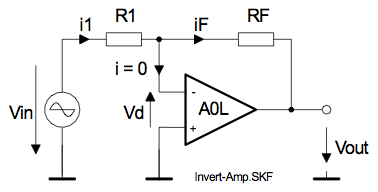
\includegraphics[width=6cm]{./images/i-verstaerker.png}
      \end{minipage}\\
\hrule
      
	\subsubsection{Nichtinvertierender Verstärker}
			Beim nichtinvertierenden Verstärker ist die Ausgangsspannung
      gleichphasig zur Eingangsspannung.\\ 
	 \begin{minipage}[T]{12cm}
      	
        \begin{tabular}{ll}
        	Closed-Loop Gain: &
        	$A_{CL}=\frac{v_{out}}{v_{in}}=\frac{R_F}{R_1}+1$\\
        	& $v_{out} = v_{in}\cdot(\frac{R_F}{R_1}+1)$ \\
        	$i_1=\frac{v_{in}-v_d}{R_1}$ &
        	$i_F=\frac{v_{out}}{R_F+R_1}$\\
          Ausgangswiderstand des NI-Verstärkers: &
          $r_{out}=0\Omega$\\
          Eingangswiderstand des NI-Verstärkers: &
          $r_{in}=\infty$\\
          OP mit Offset: &
          $v_{out} \cong \frac{R_1+R_F}{R_1} \cdot (v_{in}-v_{offset})$\\
        \end{tabular}
        Für $R_1 \to \infty$ und $R_F \to 0$ wird der Operationsverstärker zu einem
        Buffer.          	
      \end{minipage}
			\begin{minipage}{6cm}
      	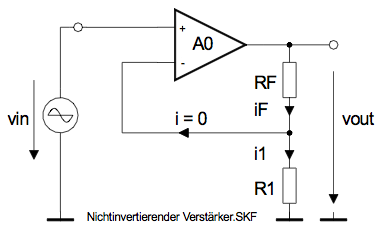
\includegraphics[width=6cm]{./images/ni-verstaerker.png}
      \end{minipage}\\
\hrule

		\begin{minipage}{12.5cm}
		\subsubsection{Verstärker mit mehreren Eingängen}
            	$A_{CL1}=-\frac{R_F}{R_1}$\\
            	$A_{CL2}=-\frac{R_F}{R_2}$\\
            	$A_{CL3}=\frac{R_F+(R_1//R_2)}{(R_1//R_2)}$\\
            	$v_{out}=A_{CL1}v_1+A_{CL2}v_2+A_{CL3}v_3=
            	-\frac{R_F}{R_1}v_1-\frac{R_F}{R_2}v_2+\frac{R_F+(R_1//R_2)}{(R_1//R_2)}v_3$\\
     	\end{minipage}
		\begin{minipage}{6cm}
      		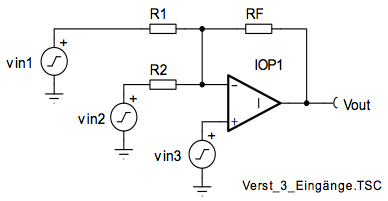
\includegraphics[width=6cm]{./images/3-eingaenge.png}
      	\end{minipage}\\
\hrule

		\begin{minipage}[c]{12cm}
		\subsubsection{Invertierender Addierer}
            $V_{out}=A_{CL1}V_{IN1}+A_{CL2}V_{IN2}+\ldots$\\
            $V_{out}=- \frac{R_F}{R_1}V_{IN1}- \frac{R_F}{R_2}V_{IN2}+\ldots$\\
            $A_{CL1}=- \frac{R_F}{R_1}$\\
           	$A_{CL2}=- \frac{R_F}{R_2}$\\
      	\end{minipage}
		\begin{minipage}{5cm}
      		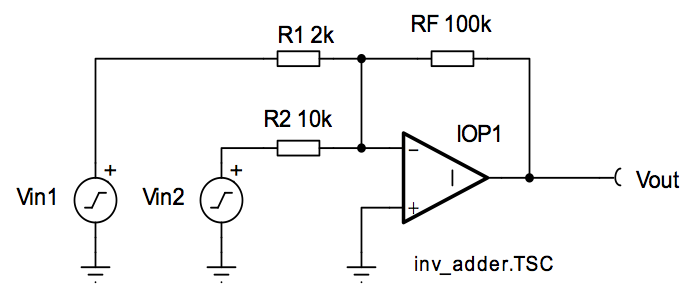
\includegraphics[width=5cm]{./images/invertadd.png}
      	\end{minipage}\\
\hrule

		\begin{minipage}[c]{12cm}
		\subsubsection{Gewichteter Subtrahierer}
            	$A_{CL1}=- \frac{R_F}{R_1}$\\
            	$A_{CL2}=
           		\frac{R_3}{R_3+R_2}\left(1+\frac{R_F}{R_1}\right)$\\
            	$v_{out}=
            	\frac{R_3}{R_3+R_2}\left(1+\frac{R_F}{R_1}\right)
            	v_{in2}-\frac{R_F}{R_1}v_{in1}$\\
      	\end{minipage}
			\begin{minipage}{5cm}
            	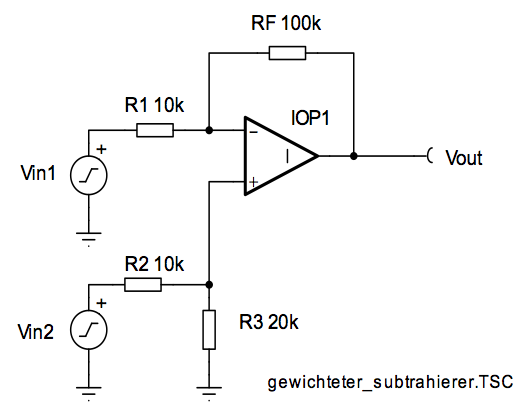
\includegraphics[width=5cm]{./images/gewichtsub.png}
            \end{minipage}\\

		\begin{minipage}[b]{12cm}
		\subsubsection{Mehrfach-Addierer-Subtrahierer} 		
			1. Man wählt $R_{F}$\\
			2. Man wählt $R_{P}$, wobei oft $R_{P}=R_{F}$ gesetzt wird. (optional)\\
			3. $R_{n}=\frac{R_{F}}{\left|A_{n}\right|}$ oder
				$R_{n}=\frac{R_{P}}{\left|A_{n}\right|}$\\ 
			4. Verstärkungsbedingung: $A_{N1} +
			\ldots + A_{Nn} = A_{P1} + \ldots + A_{Pn}$ \\Falls unerfüllt, muss ein Dummyeingang hinzugefügt werden!
		\end{minipage}
		\begin{minipage}{6cm}
          	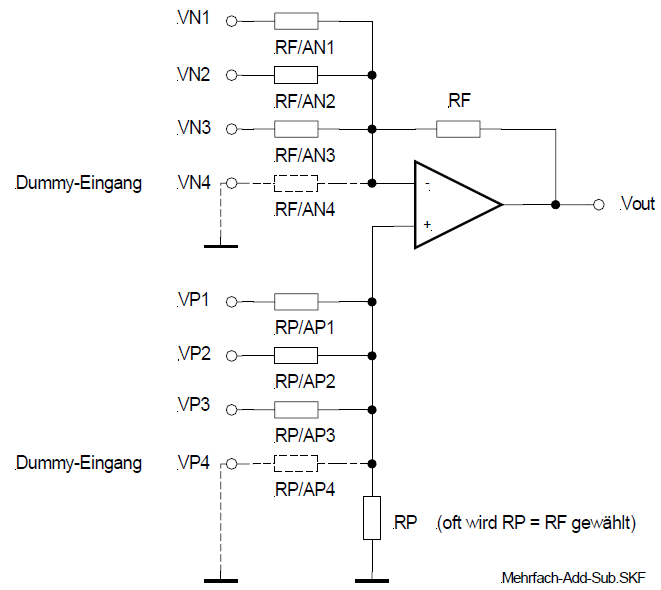
\includegraphics[width=6cm]{./images/mehrfach-addierer-subtrahierer.png} 
        \end{minipage}\\
\hrule

		\begin{minipage}[c]{12cm}
		\subsubsection{Differenzverstärker}
				Generell: \\
				$v_{out} = \frac{R_1+R_F}{R_1} \cdot (\frac{R_2}{R_2+R_3} \cdot v_{ref} + 
				\frac{R_3}{R_2+R_3} \cdot v_{in2}) - \frac{R_F}{R_1} \cdot v_{in1} $ 
				\bigskip \\
				Für $\frac{R_F}{R_1}=\frac{R_3}{R_2}$ und $v_{ref}=0V$:
				\smallskip \\
            	$A_{diff}=\frac{v_{out}}{(v_{in2}-v_{in1})}=\frac{R_F}{R_1}$\\
            	$v_{out} = \frac{R_F}{R_1}\cdot (v_{in2}-v_{in1})$\\
            \end{minipage}
			\begin{minipage}[c]{6cm}
            	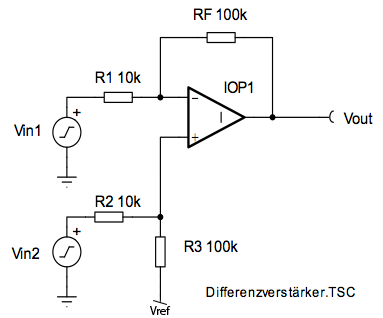
\includegraphics[width=6cm]{./images/differenzver.png}
            \end{minipage}\\
\hrule

		\begin{minipage}[c]{12cm}
		\subsubsection{Instrumentenverstärker}
			1. Stufe: Invertierender Verstärker \\
			$\Delta V_{opo}=V_{opo1}-V_{opo2}=(1+\frac{R_{F1}+R_{F2}}{R_G})\cdot(V_{in2}-V_{in1})$
			\smallskip \\
			2. Stufe: Differenzverstärker (Bedingung: $\frac{R_4}{R_3}=\frac{R_2}{R_1}$)\\
			$V_{out}=V_{ref}+\frac{R_4}{R_3}\cdot(1+\frac{R_{F1}+R_{F2}}{R_G})\cdot(V_{in2}-V_{in1})$
			\bigskip \\
			- zur Verstärkung sehr kleiner Differenzspannungen (z.B. Brückensensoren) \\
			- Oft als fertige Bauteile mit externem $R_G$ und Verstärkungen bis $1000$. \\
			\end{minipage}
			\begin{minipage}[c]{6cm}
          		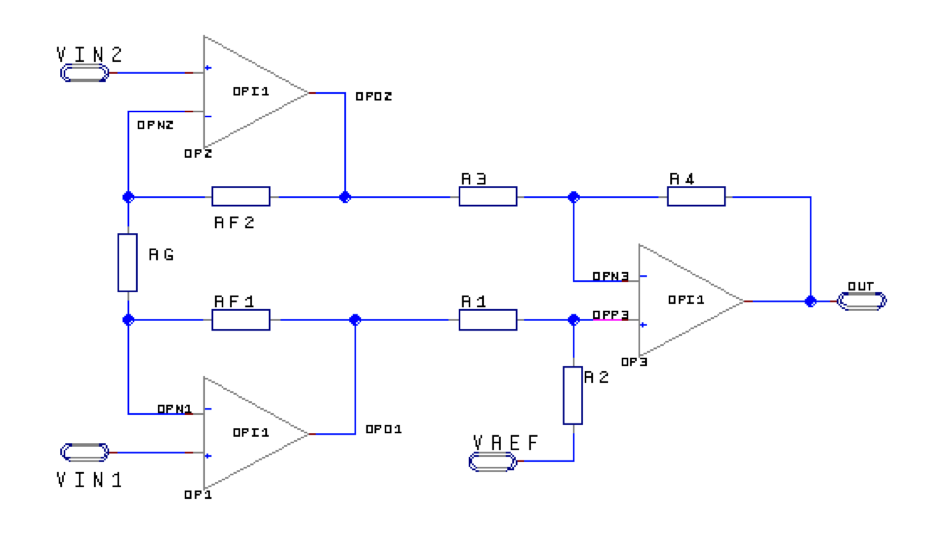
\includegraphics[width=6cm]{./images/instramp.png} 
       	 	\end{minipage}\\
\hrule     
 	 
      	 \begin{minipage}[c]{12cm}	
       	 \subsubsection{T-Glied in Rückkopplung}
       	 	Für $A \to \infty$ (idealer OP) gilt: \smallskip \\
       	 	$v_u=-\frac{R_2 \cdot R_3 + R_2 \cdot R_4 + R_3 \cdot R_4}{R_1 \cdot R_3}$
       	 	\bigskip \\
       	 	$\Longrightarrow$ hohe Verstärkung mit kleinen Wertunterschieden - 
       	 	z.B.$R_1=R_3=1k\Omega$ und $R_2=R_4=10k\Omega$ ergibt $v_u=-120$ 
       	 	(Vergleich: $v_u=-10$ bei inv. Verstärker) \\
       	 \end{minipage}
       	 \begin{minipage}[c]{5cm}
       	 	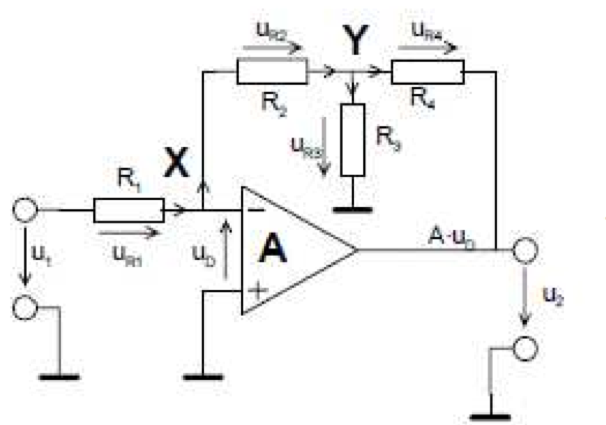
\includegraphics[width=5cm]{./images/tglied.png}
       	 \end{minipage}
\hrule      
 	 
       	 \begin{minipage}[c]{12cm}
       	 \subsubsection{Negative Impedance Converter}
       	 	Der Negative Impedance Converter (NIC) stellt einen negativen reellen Widerstand
       	 	dar. Verwendung: Kompensation parasitärer reeller Widerstände. \\
       	 	Nachteil: Masse-Bezug des negativen Widerstands. \bigskip \\
       	 	$R_{EQ}=-R \cdot \frac{R_1}{R_2}$\\
       	 \end{minipage}
       	 \begin{minipage}[c]{5cm}
       	 	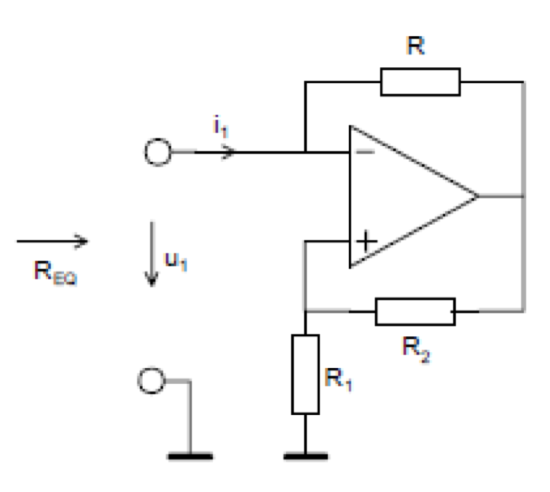
\includegraphics[width=5cm]{./images/neg-imp-conv.png}
       	 \end{minipage}
   
		\begin{minipage}[c]{12cm}        
        \subsubsection{Differentiator}
           	Beim Differentiator gilt: \\ 
           	$v_{out}=v_N-i_1 \cdot R_F$, wobei $v_N=0$ und $i_1=C_1 \cdot \frac{dv_C}{dt}$\\
           	Somit folgt:\\
           	$v_{out}=-R_FC_1 \frac{dv_{in}}{dt}$\\
           		
           	Die Elemente $C_F$ und $R_1$ sind nicht nötig, doch sie beheben eine\\
           	eine Reihe Probleme des elementaren Differentiators und fügen eine \\
           	{\bf Bandpass}-Charakteristik ein. \\
           	- Weniger Schwingneigung \\
           	- Höherer Eingangswiderstand \\
           	$\omega_1 = \frac{1}{R_1 \cdot C_1}$\\
           	$\omega_2 = \frac{1}{R_F \cdot C_F}$\\      
        \end{minipage}
		\begin{minipage}[c]{5cm}
        	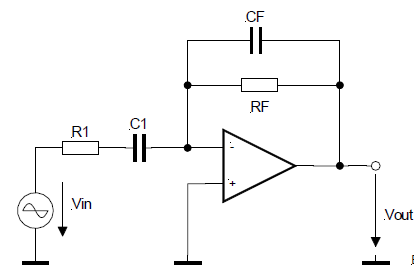
\includegraphics[width=5cm]{./images/differentiator.png}
        \end{minipage}
\hrule

		\begin{minipage}[c]{12cm}
		\subsubsection{Integrator} 
			$v_{out}=-\frac{1}{C} \int{i_C}dt + v_0$
			$v_{out}=-\frac{1}{RC} \int{v_{in}}dt +
			v_0 $\\
			$\frac{dv_{out}}{dt}=-\frac{v_{in}}{RC}$\\
			Der Widerstand $R_F$ erzeugt eine {\bf Tiefpass}-Charakteristik. \\
			Ein "Reset"-Schalter über $C$ kann Verhindern, dass der Integrator an\\
			den Anschlag läuft.
		\end{minipage} 
		\begin{minipage}[c]{5cm}
          	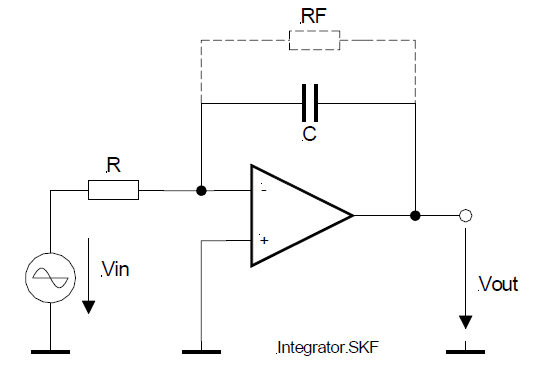
\includegraphics[width=5cm]{./images/integrator.png} 
        \end{minipage}\\
\hrule     
   
%        \subsubsection{Gesteuerte Quellen}
%			\begin{tabular}{|c|c|c|}
%				\hline
%				\multirow{2}{*}{Steuergrösse} & \multicolumn{2}{c|}{Ausgangsgrösse}\\ \cline{2-3}
%				& V & I \\ \hline
%				\multirow{8}{*}{V}	& Spannungsgesteuerte Spannungsquelle	& Spannungsgesteuerte Stromquelle		\\
%									& \bf{VCVS}								& \bf{VCCS}								\\
%									& Voltage Controlled Voltage Source		& Voltage Controlled Current Source		\\ \cline{2-3}
%									& 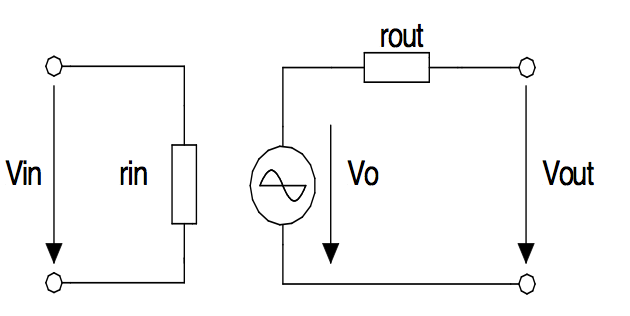
\includegraphics[width=4cm,trim=0 0 0 -5]{./images/vcvs.png}	
%									& 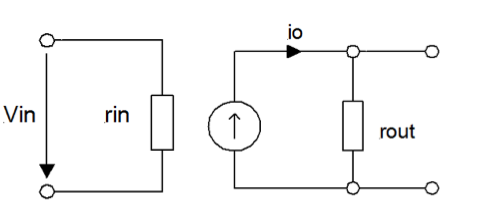
\includegraphics[width=4cm,trim=0 0 0 -5]{./images/vccs.png}					\\ \cline{2-3}
%									& $v_{out}=v_{in} \cdot A_v$			& $i_{out} = v_{in} \cdot g_m$			\\
%									& $A_v$: Spannungsverstärkung			& $g_m$: Transkonduktanz				\\ \cline{2-3}
%									& Normaler OP-Amp Verstärker
%									& 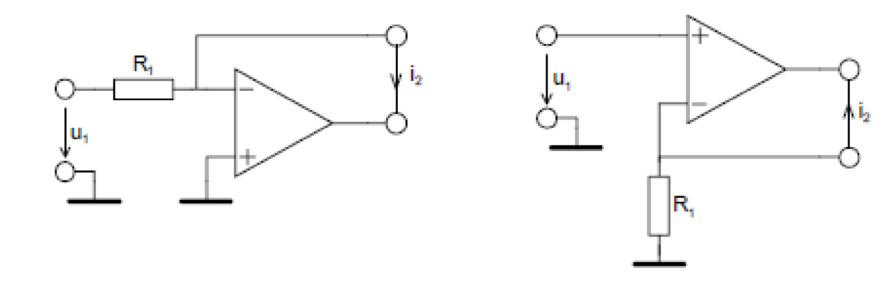
\includegraphics[width=4cm,trim=0 0 0 -5]{./images/vccs_schaltung.png}		\\
%									&	& $I_2=\frac{V_1}{R_1}$ bzw. $I_2=-\frac{V_1}{R_1}$							\\ 	\hline	
%				\multirow{8}{*}{I}	& Stromgesteuerte Spannungsquelle		& Stromgesteuerte Stromquelle			\\
%									& \bf{CCVS}								& \bf{CCCS}								\\
%									& Current Controlled Voltage Source		& Current Controlled Current Source		\\ \cline{2-3}
%									& 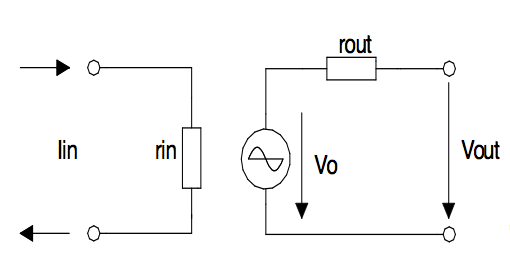
\includegraphics[width=4cm,trim=0 0 0 -5]{./images/ccvs.png}	
%									& 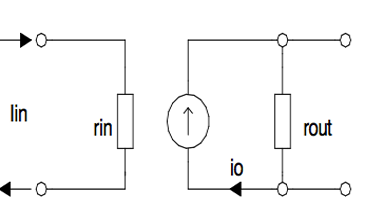
\includegraphics[width=4cm,trim=0 0 0 -5]{./images/cccs.png}					\\ \cline{2-3}
%									& $v_{out}=i_{in} \cdot r_m$			& $i_{out} = i_{in \cdot A_i}$			\\
%									& $r_m$: Transimpedanz					& $A_i$: Stromverstärkung				\\ \cline{2-3}
%									& 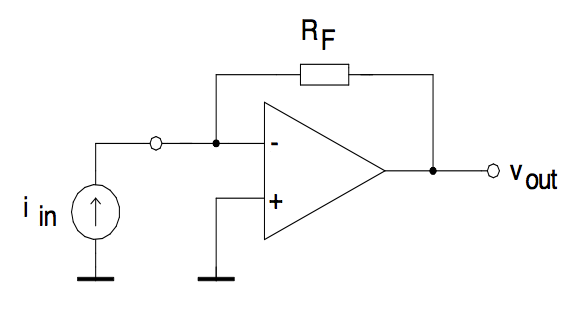
\includegraphics[width=4cm,trim=0 0 0 -5]{./images/tia.png}
%									& 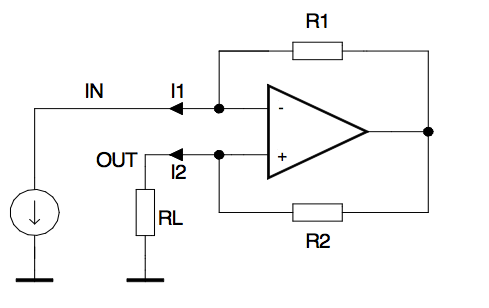
\includegraphics[width=4cm,trim=0 0 0 -5]{./images/cccs-schaltung.png}		\\ 
%									& $v_{out}=-i_{in} \cdot r_F$			& $A_i=\frac{I_2}{I_1}=\frac{R_1}{R_2}$	\\ \hline
%									
%				
%			\end{tabular} \\	
		
		\begin{minipage}[c]{12cm}	
		\subsubsection{Komparatorschaltung}
				Nicht-invertierender Komparator \\	
            	\begin{tabular}{|l|l|} \hline
            		$V_{in} > V_{ref} \pm V_{os}$ & $V_{out} = V_{out_{max}} = V_{pos}-V_{rail}$ \\
            		$V_{in} < V_{ref} \pm V_{os}$ & $V_{out} = V_{out_{min}} = V_{neg}+V_{rail}$ \\ \hline
            	\end{tabular} \\
            	
            	Invertierender Komparator \\
            	\begin{tabular}{|l|l|} \hline
            		$V_{in} > V_{ref} \pm V_{os}$ & $V_{out} = V_{out_{min}} = V_{neg}+V_{rail}$ \\
            		$V_{in} < V_{ref} \pm V_{os}$ & $V_{out} = V_{out_{max}} = V_{pos}-V_{rail}$ \\ \hline
            	\end{tabular}
			\end{minipage}
			\begin{minipage}[c]{6cm}
            	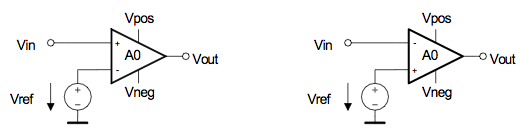
\includegraphics[width=4cm]{./images/komparator.png} \\
            \end{minipage}
\hrule

	\subsection{Schmitt-Trigger}
        \subsubsection{Nicht invertierender Schmitt-Trigger}
			\begin{minipage}[T]{13cm}
                obere Schaltschwelle
                \hspace{10.8mm}\fbox{$V_{T+} = V_{ref}\cdot \frac{R_1+R_f}{R_f}-V_{out_{min}}\cdot\frac{R_1}{R_f}$}\\
                untere Schaltschwelle
                \hspace{9.6mm}\fbox{$V_{T-} = V_{ref}\cdot \frac{R_1+R_f}{R_f}-V_{out_{max}}\cdot\frac{R_1}{R_f}$}\\
                Hysteresespannung
                \hspace{12.8mm}\fbox{$V_{H} = V_{T+}-V_{T-} = (V_{out_{max}}-V_{out_{min}})\cdot\frac{R_1}{R_f}$}\\
            \end{minipage} 
            \begin{minipage}{6cm}
                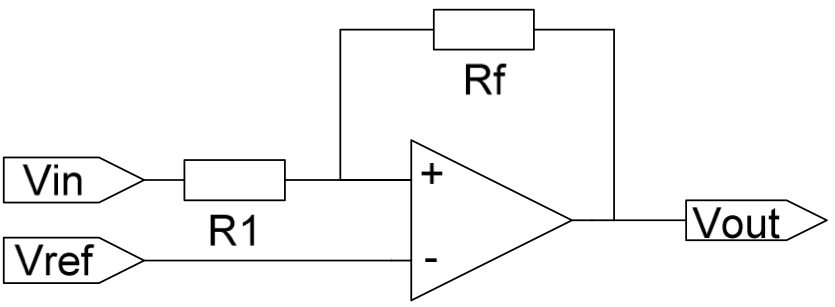
\includegraphics[width=6cm]{./images/n-schmitt.png} 
            \end{minipage}\\
            
        \subsubsection{Invertierender Schmitt-Trigger}
            \begin{minipage}[T]{13cm}
                obere Schaltschwelle
                \hspace{10.8mm}\fbox{$V_{T+} = \frac{V_{ref}\cdot R_f+ V_{out_{max}}\cdot R_1}{R_1+R_f}$}\\
                untere Schaltschwelle
                \hspace{9.6mm}\fbox{$V_{T-} = \frac{V_{ref}\cdot R_f+ V_{out_{min}}\cdot R_1}{R_1+R_f}$}\\
                Hysteresespannung
                \hspace{12.8mm}\fbox{$V_{H} = V_{T+}-V_{T-} = (V_{out_{max}}-V_{out_{min}})\cdot\frac{R_1}{R_1+R_f}$}\\
            \end{minipage} 
            \begin{minipage}{6cm}
                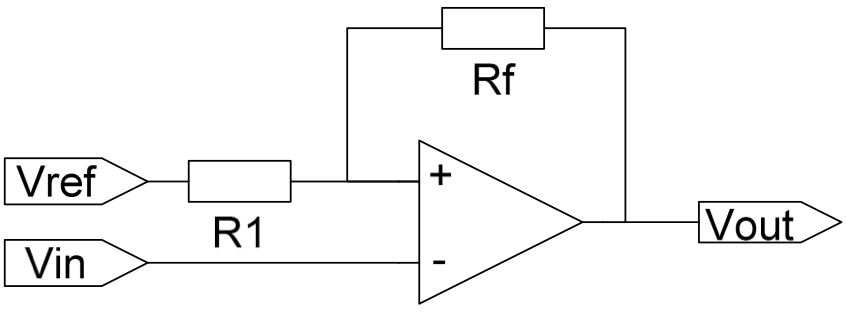
\includegraphics[width=6cm]{./images/i-schmitt.png} 
            \end{minipage}\\
            
        \subsubsection{Invertierender Schmitt-Trigger mit freien Schwellen}
        \begin{minipage}[T]{13cm}
            Schaltschwelle
            \hspace{20.8mm}\fbox{$V_{opp} =V_{ref}\cdot \frac{(R_f//R_0)}{R_1 +(R_f//R_0)}+V_{out}\cdot\frac{(R_1//R_0)}{R_f+(R_1//R_0)}$}\\
            
            Dimensionierung des Schmitt-Triggers: (Gegeben: $V_{ref}$, $V_{T+}$, $V_{T-}$)\\
            1. $V_{out_{max}}$ und $V_{out_{min}}$ ermitteln aus Datenblatt (meistens $V_{DD}$, $GND$)\\
            2. $R_f$ w\"ahlen: typisch $100 k\Omega$\\
            3. Widerst\"ande $R_1$ und $R_0$ dimensionieren\\
        \end{minipage} 
        \begin{minipage}{6cm}
            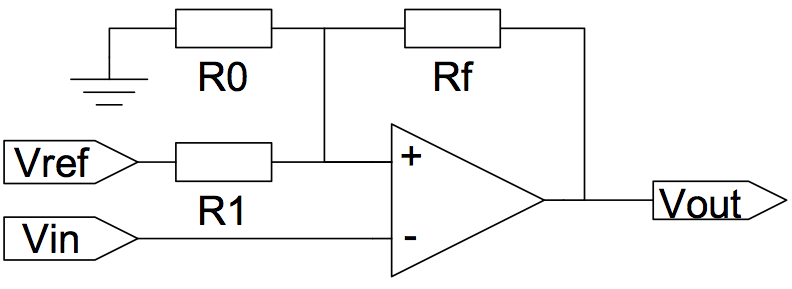
\includegraphics[width=6cm]{./images/i-schmittFreieSchwellen.png} 
        \end{minipage}\\


	\subsection{Fehlereinflüsse des Opamp}
		\subsubsection{Verstärkungsfehler bei endlicher Closed-Loop-Verstärkung}
			\begin{minipage}{12cm}
				\begin{tabular}{ll}
               	beim nichtinvertierenden Verstärker &
               	$A_{CL \hspace{1mm} ideal}=\frac{R_F}{R_1}+1$\\
               	beim invertierenden Verstärker &
                $A_{CL \hspace{1mm}
               	ideal}=-\frac{R_F}{R_1}$\\
         \end{tabular}
               	Beim invertierenden Verstärker ist eine kleine Korrektur
               	anzubringen: \\
               	$\frac{1}{A_{CL \hspace{1mm}
               	real}}=\frac{1}{A_{CL \hspace{1mm} real}}+\frac{1}{nA_{OL}}$\\
	        \end{minipage}
			\begin{minipage}{6cm}
               	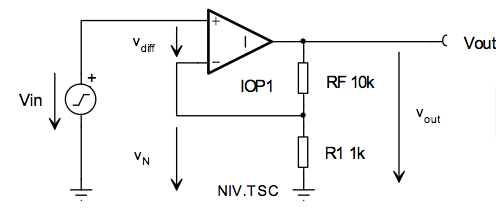
\includegraphics[width=6cm]{./images/verstaerkungsfaktor.png}
            \end{minipage}
		\subsubsection{Offsetspannungsfehler}
				\begin{tabular}{ll}
					Im Closed-Loop-Betrieb ist die Ausgangs-Fehlerspannung: &
					$V_{out \hspace{1mm}E}=V_{OS}\left( 1+\frac{R_F}{R_1}\right)$\\
          allgemein: &
          $V_{out \hspace{1mm}E}=V_{OS} \cdot {A_{CL}}^{+}$\\
          Im Open-Loop-Betrieb ist die Ausgangs-Fehlerspannung: &
          $V_{out \hspace{1mm}E}=V_{OS}\cdot {A_{CL}}^{+}$\\
          Typische Offsetspannung: & $V_{OS} \approx 0.5 \dots 5 \; mV$
         \end{tabular}
		
		\subsubsection{Eingangsstromfehler}
			\begin{minipage}{18cm}
              Wenn die Opamp-Eingangsströme gleich gross sind
              ($I_{N}=I_{P}$) und die Gleichstromwiderstände,
              die von jedem Opamp-Eingang nach Masse führen, 
              ebenfalls gleich gross gewählt werden, heben sich die
              Ausgangsspannungsfehler, die durch $I_{N}$ und $I_{P}$
              erzeugt werden, gegenseitig auf. \\
              \begin{tabular}{ll}
              Allgemeine Formel für den
              Eingangsstromfehler: &
              $V_{out \hspace{1mm}E}=I_N R_F-R_2 I_P\left( 1+\frac{R_F}{R_1} \right)$\\
              Widerstandsbedingung für Eingangsstromkompensation:&
              $R_2=\frac{R_F R_1}{R_F+R_1}=R_F // R_1$\\
              Typischer Eingangsstromfehler: & $I_E=\frac{I_P+I_N}{2}\approx 20 \dots 200 \; nA$ \\
            	\end{tabular}
            \end{minipage}\\
			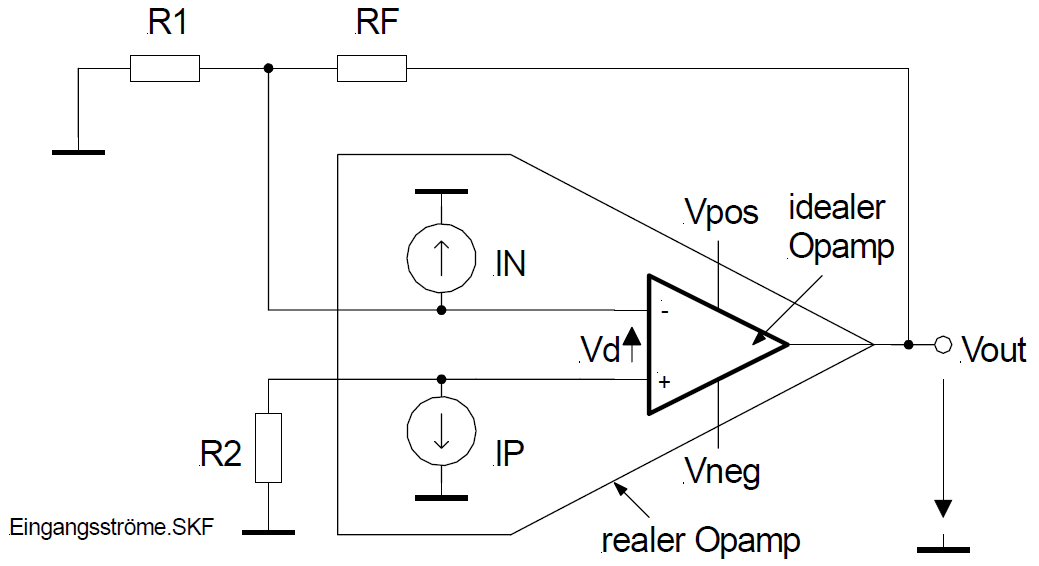
\includegraphics[width=8cm]{./images/eingangsstromfehler.png}

		\subsubsection{Eingangsstromkompensation ohne AC-Zweige}
			\begin{minipage}[b]{6cm}
            	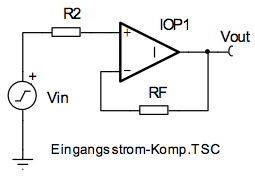
\includegraphics[height=3cm]{./images/spannungsfolger.png}\\
            	\centerline{{\bf Spannungsfolger}}\\ \\
            	$R_2$ sei ein gegebener Quellen-Widerstand\\
            	{\bf $R_F$ muss eingefügt werden}\\ \\
            	$R_F=R_2$
            \end{minipage}\hfill
			\begin{minipage}[b]{6cm}
            	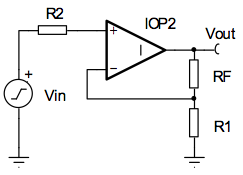
\includegraphics[height=3cm]{./images/nichtinver}\\
            	\centerline{{\bf Nichtinvertierender Verstärker}}\\ \\
            	Hier sei der Quellenwiderstand
            	vernachlässigbar.\\ {\bf $R_2$ muss eingefügt werden}\\ \\
            	$R_2=R_F//R_1$
            \end{minipage}\hfill
			\begin{minipage}[b]{6cm}
            	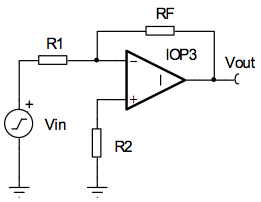
\includegraphics[height=3cm]{./images/inver}\\
            	\centerline{{\bf Invertierender Verstärker}}\\ \\ \\ \\
            	{\bf $R_2$ muss eingefügt werden}\\ \\
            	$R_2=R_F//R_1$
            \end{minipage}
			\begin{minipage}{18cm}
            	\vspace{3mm}
				\textbf{Ausgangsspannungsfehler} auf Grund des \textbf{Offsetstromes} (nur bei
				Kompensation(!)):
				\fbox{$V_{out \hspace{1mm}E}=\left|I_{OS}\right| \cdot R_F$}\\
			\end{minipage}

		\subsubsection{Power Supply Rejection Ratio PSRR}
		Schwankungen der Speisespannungen können zu Offset am Ausgang führen.
		Der PSRR beschreibt Unterdrückung solcher Beeinflussungen. \bigskip \\
		$PSRR_{lin}=\frac{dV_{supply}}{dV_{os}}$ \bigskip \\
		Meist kein Problem dank Stützkondensatoren. 
		Allenfalls Probleme bei hohen Frequenzen.
		
		\subsubsection{Common Mode Rejection Ratio CMRR}
		Schwankungen der Eingangsspannungen können am Ausgang einen Offset verursachen. \bigskip \\
		$CMRR_{lin}=\frac{dV_{CM}}{dV_{os}}$ mit $V_{CM}=V_{opp}=V_{opn}$ \bigskip \\
		Bei invertierenden Verstärkern irrelevant, da $V_{opn}=\text{konst}=V_{AGND}$.

		\subsubsection{Zusammenfassung aller Fehlereinflüsse}
      $V_{out\hspace{1mm}E\hspace{1mm}total}=A_{CL+}\cdot\left[\left|V_{OS}\right|+\frac{\left|V_{CM}\right|}{CMRR}
            	+\frac{\left|\Delta V_{Supply}\right|}{PSRR}\right]+\left|I_{OS}\right|R_F$\\

	\subsection{Dynamische Eigenschaften des Opamp}
		\begin{tabular}{ll}
			dB-Verstärkung:&
			$A_{dB}=20 \cdot log A_{lin}$\\
			lineare Verstärkung:&
			$A_{lin}=10^{\frac{A_{dB}}{20}}$\\
		\end{tabular}
		Verstärkungs-Bandbreite-Produkt GBP (Gain-Bandwidth-Product)\\
		\begin{tabular}{ll}
			Bandbreite des gegengekoppelten {\it nichtinvertierenden} Verstärkers:&
			$f_{CL+}=\frac{GBP}{A_{CL \hspace{1mm}lin}}$\\
			Bandbreite des gegengekoppelten {\it invertierenden} Verstärkers: &
			$f_{CL}=\frac{GBP}{\left| A_{CL \hspace{1mm}lin}\right|+1}$\\
		\end{tabular}\\
		{\bf Gesetz vom Konstanten Verstärkungs-Bandbreite-Produkt:} \\
		Für jeden Punkt auf der mit -20dB abfallenden Frequenzgang-Gerade ist das
		Produkt aus Verstärkung und zugehöriger Frequenz konstant gleich GBP, d.h. $A_{lin}\cdot f=GBP=konst$\\
		\subsubsection{Slew-Rate}
			\begin{tabular}{ll}
				min. SR bei einem Sprungsignal &
				$SR\geq\frac{0.8V_{step}}{t_{anstieg}}$\\ 
				min. SR bei einem Sinussignal & 
				$SR\geq V_{amplitude}\omega=V_{amplitude}2\pi f$\\
				typische Slew-Rate: & $SR \approx 0.5 \dots 50 \frac{V}{\mu s}$
			\end{tabular}

			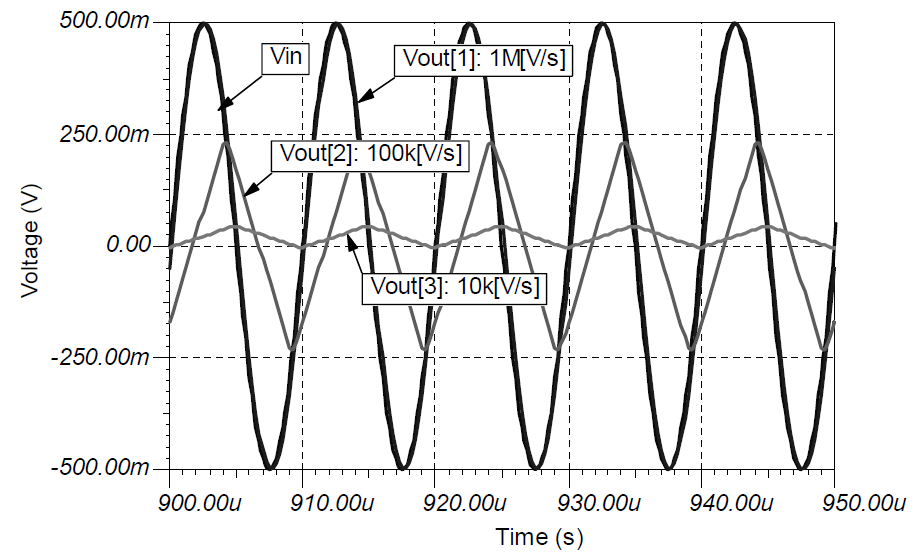
\includegraphics[height=5cm]{./images/slew-rate.png}\\

			{\bf Anstiegszeit des Ausgangs:} \\
			\begin{tabular}{ll}
				$t_{rout}$ & = $\sqrt{t_{rin}^2 + t_{rAmp}^2}$ \\
				$t_{rin}$  & = Anstiegszeit des Eingangssignals \\
				$t_{rout}$ & = Anstiegszeit des Ausgangssignals \\
				$t_{rAmp}$ & = $\frac{0.35}{f_{bw}} = $ Eigenanstiegszeit des Verstärkers \\
				$f_{bw}$   & = Kleinsignalbandbreite des Verstärkers \\
			\end{tabular}

